\documentclass{beamer}

\usepackage[utf8]{inputenc}

\title{\Huge \textbf{Control Systems-EE2101}\newline\large\textit{Assignment 1}}

\author{{\LARGE \textbf{Abhijeet Gunjal} \newline{ME18BTECH11001}}}
\institute{\large\newline IITH}
\date{9th September 2020}

\begin{document}

\frame{\titlepage}

\begin{frame}
\begin{center}
\frametitle{\textbf{\Huge CHAPTER 2}}
\textbf{\Large Practice Problem 62}\newline
\end{center}
Figure shows a crane hoisting a load. Although the actual system's model is highly non-linear, if the rope is considered to be stiff with a fixed length L, the system can be modelled using the following equations:
\newline\newline
\begin{center}
$m_L\"{x}_{La} = m_Lg\phi$
\newline
$m_T\"{x}_T = f_T - m_Lg\phi$
\newline
$x_{La} = x_T - x_L$
\newline
$x_L = L\phi$
\newline
\end{center}
\end{frame}

\begin{frame}
\newline
where $m_L$ is the mass of the load, $m_T$ is the mass of the cart, $x_T$ and $x_L$ are displacements as defined in the figure, $\phi$ is the rope angle with respect to the vertical, and $f_T$ is the force applied to the cart(Marttinen, 1990).
\newline
\textbf{a.} Obtain the transfer function from cart velocity to rope angle $\frac{\Phi(s)}{V_T(s)}$.
\newline
\textbf{b.} Assume that the cart is driven at a constant velocity $V_0$ and obtain an expression for the resulting $\phi(t)$. Show that under this condition, the load will sway with a frequency $\omega_0 = \sqrt{\frac{g}{L}}$.
\newline
\textbf{c.} Find the transfer function from the applied force to the cart's position, $\frac{{X_T(s)}{F_T(s)}}$.
\newline
\textbf{d.} Show that if a constant force is applied to the cart, its velocity will increase without bound as $t \to \infty$.
\end{frame}

\begin{frame}
\begin{figure}[H]
\centering
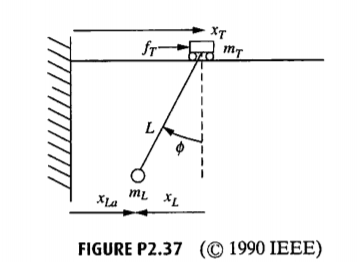
\includegraphics[height=1.5in]{Figure.png}

\end{figure}
\end{frame}

\begin{frame}{\textbf{\Huge Solution}}
\newline\textbf{a.}
\newline We have that  
$m_L\"{x}_{La} = m_Lg\phi$
\newline
$x_{La} = x_T - x_L$
\newline
$x_L = L\phi$\newline
From the second equation,\newline
$\"x_{La} = \"x_T - \"x_L = \.v_T - L\ddot{\phi}= g\phi$\newline\newline
Obtaining Laplace transforms on both sides of the previous equation\newline
$sV_T - Ls\Phi = g\Phi$ from which $sV_T = \Phi(g + Ls^2)$
\newline
so that\newline\newline
$\frac{\Phi}{V_T}(s) = \frac{s}{g+Ls^2} = \frac{1}{L}\frac{s}{s^2 + \frac{g}{L}} = \frac{1}{L}\frac{s}{s^2 + \omega_0^2}$

\end{frame}

\begin{frame}
\newline\textbf{b.}
\newline
Constant velocity $V_T(s) = \frac{V_0}{s}$ so the angle is\newline\newline$\Phi(s) = \frac{V_0}{L}\frac{1}{s^2 + \omega_0^2}$
\newline\newline
Obtaining inverse Laplace transform,\newline\newline
$\phi(t) =\frac{V_0}{L\omega_0}sin(\omega_0t)$, the load will sway away with a frequency $\omega_0$.

\end{frame}

\begin{frame}
\newline\textbf{c.}\newline
From $m_T\ddot{x_T} - f_T - m_Lg\phi$ and Laplace transformation, we get\newline\newline 
$m_Ts^2X_T(s) = F_T - m_Lg\Phi(s)$\newline\newline
$ = F_T - m_Lg\frac{1}{L}\frac{s}{s^2 + \omega_0^2}V_T$
$ = F_T - m_Lg\frac{1}{L}\frac{s^2}{s^2 + \omega_0^2}X_T$
\newline\newline
From which\newline\newline
$\frac{X_T}{F_T} = \frac{1}{s^2(m_T + \frac{m_Lg}{L}\frac{1}{s^2 + \omega_0^2})}$
$ = \frac{s^2 + \omega_0^2}{s^2(m_T(s^2 + \omega_02) + m_L\omega_0^2)}$
$ = \frac{1}{m_T}\frac{s^2 + \omega_0^2}{s^2(s^2 + a\omega_0^2)}$
\newline\newline
where, \newline \newline
$a = 1 + \frac{m_L}{m_T}$
    
\end{frame}


\begin{frame}
\newline\textbf{d.}\newline
From part c,\newline\newline
$\frac{V_T}{F_T} = \frac{sX_T}{F_T} = \frac{1}{m_T}\frac{s^2 + \omega_0^2}{s^2(s^2 + a\omega_0^2)}$\newline\newline
Let $F_T = \frac{F_0}{s}$ then,\newline\newline
$V_T(s) = \frac{F_0}{m_t}\frac{s^2 + \omega_0^2}{s^2(s^2 + a\omega_0^2)} = \frac{A}{s^2} + \frac{B}{s} + \frac{Cs + D}{s^2 + a\omega_0^2}$\newline\newline
After partial fraction expansion,\newline\newline
$v_T(t) = A't + B + C'cos(a\omega_0t + \theta$\newline\newline
From which, it is clear that 
$v_T \to \infty$ as $ t \to \infty$
\newline\newline
Hence If constant force is applied, the velocity of cart will increase boundless with time.


\end{frame}
\end{document}
